\documentclass[12pt]{amsart}

\addtolength{\hoffset}{-2.25cm}
\addtolength{\textwidth}{4.5cm}
\addtolength{\voffset}{-2.5cm}
\addtolength{\textheight}{5cm}
\setlength{\parskip}{0pt}
\setlength{\parindent}{15pt}

\usepackage{amsthm}
\usepackage{amsmath}
\usepackage{amssymb}
\usepackage[colorlinks = true, linkcolor = black, citecolor = black, final]{hyperref}

\usepackage{graphicx}
\graphicspath{ {./images/} }
\usepackage{multicol}
\usepackage{ marvosym }
\usepackage{wasysym}
\usepackage{tikz}
\usetikzlibrary{patterns}

\newcommand{\ds}{\displaystyle}
\DeclareMathOperator{\sech}{sech}

\setlength{\parindent}{0in}

\begin{document}

\thispagestyle{empty}

{\scshape Sotirios Moschos 9030} \hfill {\scshape \large Advanced Signal Processing} \hfill {\scshape Homework \#2}

\smallskip

\hrule

\bigskip

{\large\textbf{Plots}}

\textbf{Real discrete process X(k)}
\begin{figure}[h]
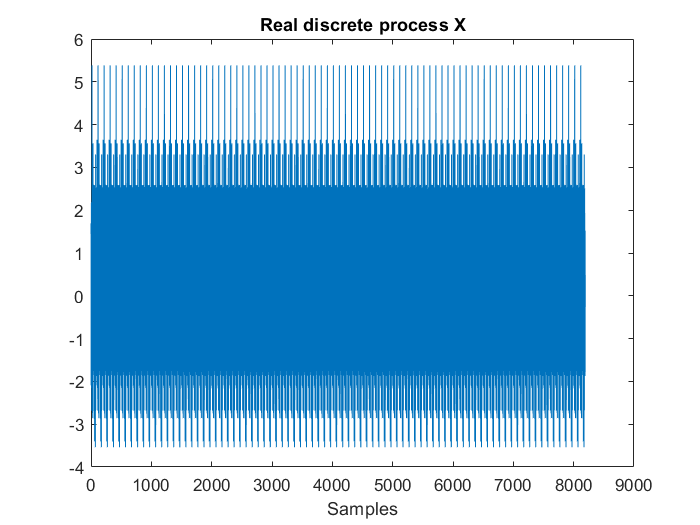
\includegraphics[width=8cm]{{Images/X(k).png}}
\end{figure}

In order to get the power spectrum we used the function SpectrumEstimator from the dsp toolbox.
We chose Welch's averaged modified periodograms method and Hann's window function.

\textbf{Power spectrum 1}
\begin{figure}[h]
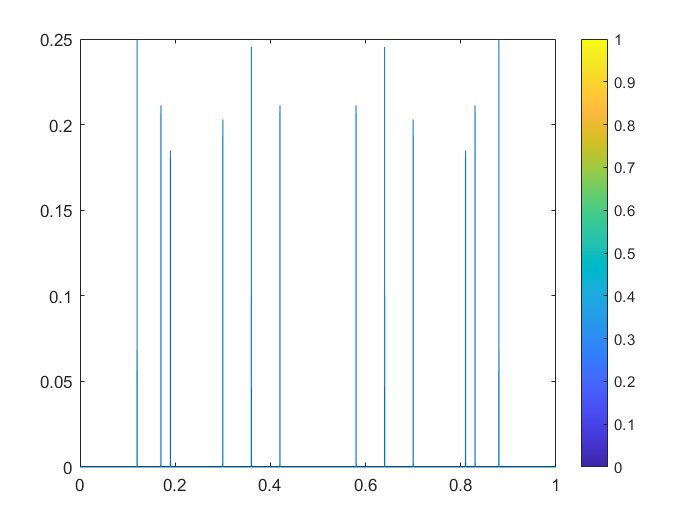
\includegraphics[width=8cm]{{Images/power spectrum 1.png}}
\end{figure}

In another approach, we calculated the the power spectrum via the FFT of the covariance of X(k). Hence, we got the following plot.

\textbf{Power spectrum 2}
\begin{figure}[h]
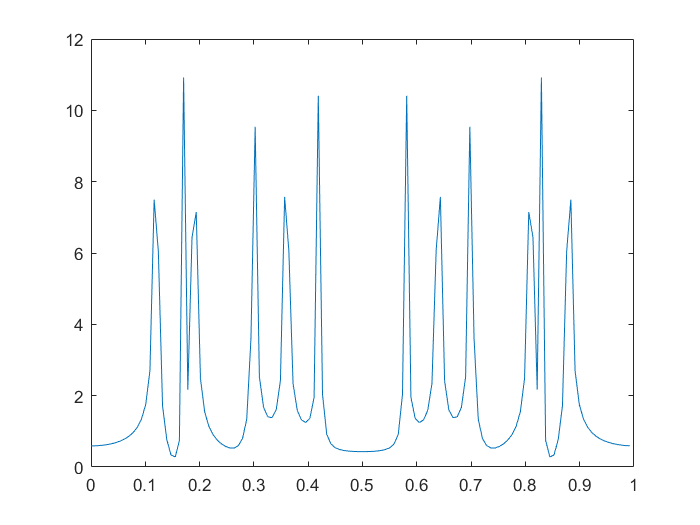
\includegraphics[width=8cm]{{Images/power spectrum 2.png}}
\end{figure}

\bigskip

{\large\textbf{Comparison of indirect bispectrum estimation methods}}

\bigskip

In order to get the following plots, we used the bispeci function from HOSA toolbox. For the first subtask we used the hexagonal window with unity values, as it's shape is similar to the rectangular window, so we can draw similar conjectures.\newline
For the second subtask we used the parzen window.\newline
Hence, we got the following plots: For the first plot we used the hexagonal window with unity values and for the second plot the parzen window.
\begin{figure}[h]
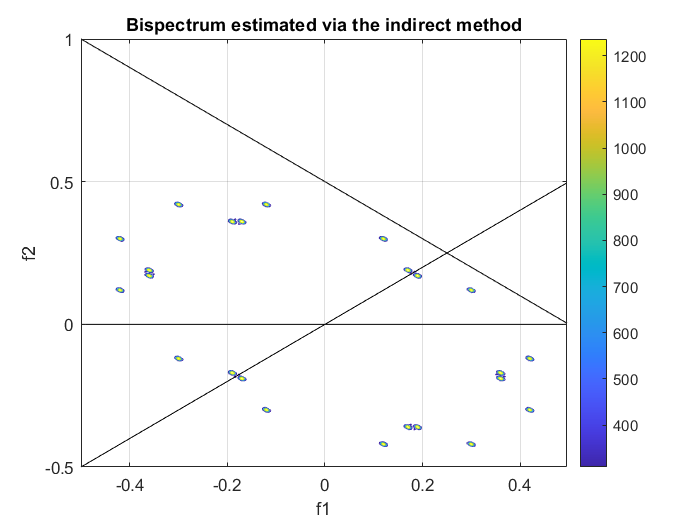
\includegraphics[width=8cm]{{Images/indirect method-hexagonal uniform window.png}}
\end{figure}
\begin{figure}[h]
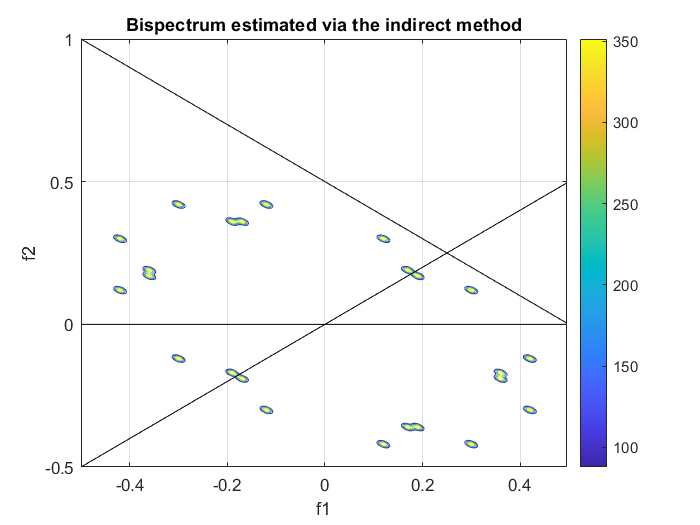
\includegraphics[width=8cm]{{Images/indirect method-parzen window.png}}
\end{figure}

For the exact explanation, check this paper, which analyses the comparison of windows  (\textbf{Bispectral resolution and leakage effect of the indirect bispectrum estimate for different types of 2D window functions, 2008, Teofil-Cristian Oroian et all.}).

\bigskip
\newpage
{\large\textbf{Comparison of indirect and direct bispectrum estimation methods}}

\bigskip

In order to get the following plot, we used the bicpecd function from HOSA toolbox.
\begin{figure}[h]
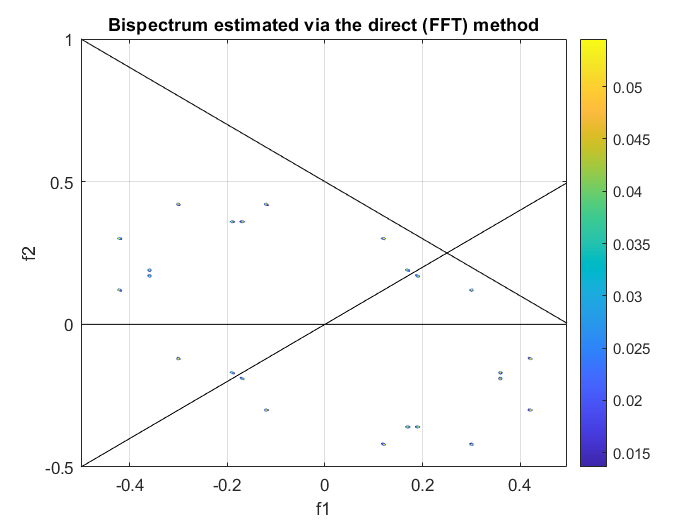
\includegraphics[width=8cm]{{Images/direct method.png}}
\end{figure}\newline
Need to add an explanation about indirect and direct method.

\bigskip

{\large\textbf{Frequency content of power spectrum vs bispectrum estimations}}


\end{document}
